\documentclass[aps,pre,preprint,superscriptaddress,nofootinbib]{revtex4-2}
\usepackage{amsmath,amssymb,graphicx,booktabs,array,microtype,hyperref}
\usepackage[T1]{fontenc}
\usepackage{lmodern}
\hypersetup{colorlinks=true,linkcolor=blue,citecolor=blue,urlcolor=blue}
\newcommand{\Vcal}{\mathcal{V}}
\newcommand{\Cdyn}{C_{\mathrm{dyn}}}
\newcommand{\Bin}{B_{\mathrm{in}}}
\begin{document}

\title{From Trace to Modal Closure: Dynamic Conditions for Regenerative Reentry in a Path-Dependent Adaptive System}
\author{Gregorio Rozas Fern\'andez}
\affiliation{Independent Researcher}
\date{October 4, 2026}

\begin{abstract}
Historical information can remain causally available in an adaptive dynamical system without being reusable across repeated transmissions. We study this distinction in a simulated nonlinear recurrent system containing fast recurrent state, slow memory variables, relevance, boundary, and plasticity traces. Common-present interventions show that prior histories remain causally active after the fast carrier has been matched, with historical information distributed across variables and expressed context dependently through collective readout. An isolated recurrent-state $\rightarrow$ memory $\rightarrow$ recurrent-state relay is causal but strongly dissipative: its maximum local singular gain is approximately $0.10$, and even its optimally transmitted input direction returns along a substantially different output direction. One-pass modal selection therefore does not imply reproduction of the selected mode.

We define \emph{modal closure} operationally as an output-to-input geometric compatibility condition for repeated use of a transmission channel. Tested native co-products, common cross-instance maps, and simple static architectural hypotheses do not supply this closure. In contrast, a closure map reconstructed from the instance-specific effective causal write and return operators transfers from one calibration context to a distinct test context with mean absolute directional alignment $0.999763$. When this fixed external closure is combined with a fixed scalar gain normalization, and neither component is recomputed, the nonlinear relay preserves near-unit packet amplitude over four tested generations ($0.99213$ at generation 4), whereas the same fixed gain without geometric closure falls to $0.07959$. Nonorthogonal mixed packets are also progressively enriched toward the compatible mode, while an exactly orthogonal packet is not immediately attracted.

The result is deliberately limited: externally supplied modal closure plus fixed gain is sufficient for finite-horizon regenerative reentry in the tested system. The reactor does not learn the closure map or gain, and the experiments do not establish autonomy, autopoiesis, subjective experience, or asymptotic stability.
\end{abstract}

\maketitle

\section{Introduction}

A dynamical system may carry a trace of its past without being able to use that trace repeatedly. This distinction is easy to obscure when memory is operationalized only as delayed decodability, persistent state, or one-pass influence on future behavior. Dynamical-systems accounts have shown how past inputs can be retained in transient state, distributed modes, or non-normal recurrent dynamics \cite{Ganguli2008,Goldman2009,Trefethen2005}. Reservoir and liquid-state approaches likewise exploit transient recurrent responses without requiring convergence to a task-specific stable state \cite{Maass2002,JaegerHaas2004,Lukosevicius2009}. Context-dependent recurrent computation, mixed selectivity, and trained recurrent trajectories further demonstrate that latent structure can be expressed differently depending on present state and recurrent dynamics \cite{Mante2013,Rigotti2013,Sussillo2009,Laje2013}. These results motivate a sharper question: what additional condition is needed when a returned signal must remain usable by the same channel again?

The present study separates four properties that are often conflated. A \emph{trace} means that historical differences remain causally available at a matched present. \emph{Reentry} means that perturbing one state family leaves a causal effect in another family and can later return to the original family. \emph{Selection} means that some component is preferentially transmitted during one passage. \emph{Regeneration}, as used here, means only that transmissible organization persists through a finite sequence of externally corrected passages. This last term does not imply energetic autonomy, autopoiesis, endogenous learning, or biological self-maintenance.

The distinction matters especially in non-normal systems. A channel can amplify or preferentially transmit an input direction while rotating it into a different output direction \cite{Trefethen2005,Hennequin2014}. If the output of one passage is poorly aligned with the input geometry favored by the next, scalar gain compensation can preserve magnitude without preserving reusability. Repeated transmission then fails even though every individual passage contains a well-defined optimal mode.

We investigate this problem in a path-dependent adaptive reactor with coupled fast and slow variables. The study follows a causal sequence:
\begin{equation}
\begin{aligned}
\text{history}&\rightarrow\text{distributed trace}\rightarrow\text{contextual readout}\rightarrow\text{reentry}\rightarrow\text{selection}\\
&\rightarrow\text{modal mismatch}\rightarrow\text{closure}\rightarrow\text{finite-horizon regenerative reentry}.
\end{aligned}
\end{equation}
The central mathematical step is elementary linear algebra: for a fixed channel $T=U\Sigma V^T$, an output-to-input partial isometry $C=VU^T$ converts transmitted output modes back into compatible input modes. Orthogonal frame matching, Procrustes constructions, and polar factors are classical \cite{Schonemann1966,Higham1986}; likewise, input--output gain and system-identification frameworks provide established languages for reasoning about transmission and locally inferred dynamics \cite{Zames1966,Ljung1999,Schmid2010}. We do not claim a new matrix decomposition or invoke a small-gain theorem as a proof of the nonlinear result. The scientific question is instead whether a closure geometry can be identified from the reactor's effective causal dynamics, frozen, transferred across a context change, and shown to matter in the full nonlinear relay.

Our main result is a sufficiency result. In the tested protocol, a fixed instance-specific closure reconstructed from effective write and return operators, combined with a fixed scalar gain, supports four generations of nonlinear recurrence. Neither closure nor gain is learned by the reactor. Endogenous acquisition of these quantities is left as a separate problem.

\section{Model and methods}

\subsection{Reactor architecture}

The recurrent state is $x_t\in\mathbb{R}^{32}$, partitioned into four modules of eight units. Body, environment, and action variables are $s_t,e_t,a_t\in\mathbb{R}^{4}$; contextual state is $c_t\in\mathbb{R}^{8}$; slow memory is $m_t\in\mathbb{R}^{8}$; plastic modulation is $\theta_t\in\mathbb{R}^{4}$; relevance is $r_t\in\mathbb{R}^{12}$; the boundary trace is $K_t\in\mathbb{R}^{8\times4}$; and $b_t\in\mathbb{R}^{8}$ is a nonlinear readout of boundary-row magnitudes. A rolling history $g_h$ stores the five most recent four-dimensional vectors of recurrent module means.

The baseline recurrent matrix $W_0$ is modular and sparse, with within-module connection probability $0.35$, between-module probability $0.05$, nonzero weights drawn from $\mathcal N(0,0.35)$, and spectral radius normalized to $0.75$. The input matrix $\Bin\in\mathbb{R}^{32\times12}$ has entries $\mathcal N(0,0.18)$; the memory matrix $M\in\mathbb{R}^{32\times8}$ has entries $\mathcal N(0,0.12)$; and $P_m\in\mathbb{R}^{8\times32}$ has entries $\mathcal N(0,1/\sqrt{32})$. Four normalized sparse matrices $A_k$ modulate recurrent structure,
\begin{equation}
W(\theta_t)=W_0+\sum_{k=1}^{4}\theta_{t,k}A_k.
\end{equation}
The context matrices satisfy $S_e\sim\mathcal N(0,0.18)$, while only four randomly selected rows of $S_a$ are nonzero with entries $\mathcal N(0,0.30)$. Additional recurrent couplings $J_p,J_r,J_b$ have entrywise standard deviations $0.04$, $0.025$, and $0.025$, respectively.

Let $u_t=[s_t;c_t]$. Relevance rescales the effective input through
\begin{equation}
 u_t^{\mathrm{eff}}=u_t\odot(1+0.5\,\hat r_t),
\end{equation}
where $\hat r_t=|r_t|/\max|r_t|$ when $r_t\neq0$. Recurrent dynamics are
\begin{align}
 z_t &= W(\theta_t)x_t+\Bin u_t^{\mathrm{eff}}+Mm_t+J_pp_t^{\mathrm{pre}}+J_rr_t+J_bb_t,\\
 x_{t+1} &=0.75x_t+0.25\tanh z_t.
\end{align}
The slow memory update is
\begin{equation}
 m_{t+1}=0.98m_t+0.02P_mx_{t+1}.
\end{equation}
The boundary trace follows
\begin{equation}
 K_{t+1}=0.98K_t+0.02\,c_t\zeta_{t-1}^{T},
\end{equation}
where $\zeta$ denotes the previous action-noise vector in the recovered reactor source. Its nonlinear readout is
\begin{equation}
 b_i=\sigma\!\left(12\left[\|K_i\|-\operatorname{median}_j\|K_j\|\right]\right).
\end{equation}
The recurrent drive uses $p_t^{\mathrm{pre}}$, an exponentially weighted average of up to five module-mean vectors already present in the history deque, with weights proportional to $\exp(-\mathrm{lag}/2)$. After the new recurrent state is computed, its module-mean vector is appended and a post-update summary $p_t^{\mathrm{post}}$ is used by the C4 plasticity update.

Actions are
\begin{equation}
 a_t=\operatorname{clip}\left[\tanh(0.8s_t)+0.25\tanh(g_t)+\zeta_t,-1,1\right],
\end{equation}
and viability is
\begin{equation}
 \Vcal_t=\exp\left[-\frac{\|s_t\|^2}{2(0.35)^2}-0.05\|a_t\|^2\right].
\end{equation}
The environment and adaptive traces follow the recovered C4 source exactly. With environmental drive $\mu_t$ and $\Delta\Vcal_t=\Vcal_t-\Vcal_{t-1}$,
\begin{align}
 e_{t+1} &=0.95e_t+0.03\eta^{\mathrm{env}}_t+\mu_t,\\
 r_{t+1} &=0.98r_t+0.02u_{t-1}\Delta\Vcal_t.
\end{align}
Let $\chi_t$ be the four-vector of module-wise mean squared recurrent activity and $\chi^*$ the fixed reference target. In the C4 branch,
\begin{equation}
 \theta_{t+1}=\operatorname{clip}\!\left[\theta_t+0.002(\chi^*-\chi_{t+1})-0.004\theta_t+0.0005\,\Delta\Vcal_t p_t^{\mathrm{post}},-0.25,0.25\right].
\end{equation}
The context is $c_t=S_ee_t+S_aa_t+\eta^{c}_t$. Body noise has standard deviation $0.005$, contextual noise $0.02$, and action exploration noise $0.02$. The exact within-step update order, including the two uses of the temporal summary before and after appending the current module means, is given in the Supplement.

In the base relation branch,
\begin{equation}
 s_{t+1}=A_ss_t-0.40a_t+0.25e_t+\eta_t,
\end{equation}
where $A_s=0.94I$ plus a cyclic $0.015$ coupling. Paper-IV histories use the relational extension
\begin{equation}
 s_{t+1}=A_ss_t-0.40R_4(\phi)a_t+0.25e_t+\eta_t,
\end{equation}
where $R_4(\phi)$ is the same planar rotation applied to body/action coordinate pairs $(1,2)$ and $(3,4)$. The reference implementation released with this paper fixes its sign convention from the prospectively frozen causal-signature estimator and passes the angle-recovery self-check across the audited relation angles. It is labeled as a reconstruction rather than as a byte-identical recovery of the transient original source.

\subsection{Common-present tests and historical supports}

The common-present protocol asks whether histories remain causally active after fast/current variables are matched. In the first exact protocol, 12 relation histories spanning $-150^\circ$ to $180^\circ$ were run for 80 steps. At the common present, the fast/current carrier $[s,e,x,a,\mathrm{prev\_u},\mathrm{prev\_z},\mathrm{prev\_v}]$ was retained while the slow historical package $[m,\theta,r,K,b,g_h]$ was transplanted. All branches then received the same future relation ($\phi=0$) and the same future noise for eight steps. The response vector concatenated eight actions and eight recurrent-state increments. Later experiments used related common-carrier interventions with experiment-specific retained/transplanted sets; the released master matrix and frozen design files record the exact scope available for each branch.

Distributed-trace experiments separately intervened on $r,m,K$, and $g_h$ and quantified both response amplitude and representational similarity. Contextual-reactivation experiments crossed historical packages with eight present probes and removed history-only and present-only main effects, leaving a history-by-present interaction. Multi-trace experiments tested whether later $K$ states were explained by the correct two-trace span rather than by an unrelated span or the best single trace.

\subsection{Isolated write-return relay and local causal operators}

The principal reentry analysis isolates a 24-step recurrent-state-to-memory write phase followed by a 24-step memory-to-recurrent-state return phase. Local causal operators are estimated by central finite differences with $\epsilon=10^{-4}$ around the tested carrier:
\begin{align}
 A &= \frac{\partial m_{t+24}}{\partial x_t}\in\mathbb{R}^{8\times32},\\
 B &= \frac{\partial x_{t+48}}{\partial m_{t+24}}\in\mathbb{R}^{32\times8},\\
 T &= BA\in\mathbb{R}^{32\times32}.
\end{align}
These are intervention-defined local causal operators. They are not claimed to be global Jacobians of the full adaptive simulator.

The singular value decompositions are
\begin{equation}
 A=U_A\Sigma_AV_A^T,\qquad B=U_B\Sigma_BV_B^T.
\end{equation}
Finite-amplitude probes along the leading right singular vector of $T$ were run separately from the local finite-difference audit.

\subsection{Geometric observables}

For nonzero vectors $a,b$, directional comparisons are sign invariant:
\begin{equation}
 c_{\pm}(a,b)=\frac{|a^Tb|}{\|a\|\,\|b\|},\qquad
 \alpha_{\pm}(a,b)=\arccos c_{\pm}(a,b).
\end{equation}
For one-dimensional modal subspaces, projector displacement is
\begin{equation}
 d_P(v,w)=\|vv^T-ww^T\|_F
\end{equation}
for unit vectors $v,w$. The native interface efficiency used below is
\begin{equation}
 \eta_{\mathrm{int}}=\frac{\sigma_1(BA)}{\sigma_1(A)\sigma_1(B)}.
\end{equation}
Normalized non-normality is $\|T^TT-TT^T\|_F/\|T\|_F^2$. In the multigenerational experiments, relative amplitude is $a_g=\|d_g\|/\|d_0\|$, modal alignment is $F_g=c_{\pm}(d_g,v)$, and compatible share is $S_g=F_g^2$. Representational-similarity and closure-need definitions, including experiment-specific distance structures, are specified in the Supplement.

\subsection{Dynamic closure construction}

The effective interface between the write and return half-channels is summarized by
\begin{equation}
 H=\Sigma_BV_B^TU_A\Sigma_A,
\end{equation}
with
\begin{equation}
 H=U_H\Sigma_HV_H^T.
\end{equation}
The instance-specific dynamic closure is
\begin{equation}
 \boxed{\Cdyn=V_AV_HU_H^TU_B^T.}
\end{equation}
It maps the transmitted output frame of the return channel back toward the reusable input frame of the write channel. Closure was reconstructed in calibration context $c_A=(-135^\circ,-45^\circ,45^\circ)$ at calibration carrier $q_{\mathrm{cal}}$ and tested, without refitting, in context $c_B=(45^\circ,135^\circ,-135^\circ)$ at test carrier $q_{\mathrm{test}}$.

\subsection{Fixed gain and multigenerational relay}

The fixed scalar normalization was
\begin{equation}
 \gamma^{c_A}=\frac{1}{\sigma_1(T^{c_A})}.
\end{equation}
It was estimated once in the calibration carrier and then frozen. Each nonlinear generation consisted of a native 24-step write, scaling the newly written $\Delta m$ by $\gamma^{c_A}$, and a native 24-step return. In the local linear model this placement is exactly equivalent to loop-level scalar gain because $B(\gamma A\delta x)=\gamma BA\delta x=\gamma T\delta x$; no such global nonlinear equivalence is assumed. Where closure was enabled, the returned $\Delta x$ was transformed by the frozen $\Cdyn^{c_A}$ and renormalized to its pre-closure packet norm so that closure itself supplied no magnitude. No singular vectors, maps, or gains were recomputed during the four-generation test.

The decisive comparator, labeled \texttt{UNCORRECTED}, received the same fixed gain but no geometric closure. It is therefore a gain-compensated, geometrically unclosed control, not a fully native/no-gain branch. Additional controls used a static within-instance map or a dynamic map from the wrong reactor instance.

For projective-basin tests, initial packets were constructed at $22.5^\circ$, $45^\circ$, $67.5^\circ$, and $90^\circ$ relative to the frozen calibration input mode $v^{c_A}$, with three orthogonal directions per nontrivial angle. Compatible share was $S_g=\cos^2(d_g,v^{c_A})$.

\subsection{Design and inference}

The experiments use independent seed cohorts for the main confirmatory blocks. Frozen design JSONs were recovered for the principal late operator, closure, and regenerative-reentry experiments and for several earlier causal blocks. Because these designs were frozen prospectively inside the research record but were not deposited in an independent timestamped registry before execution, we describe them as \emph{prospectively frozen confirmatory criteria}, not as externally preregistered studies.

Inference is experiment specific and includes bootstrap confidence intervals, seed-level favorable fractions, randomization/sign-flip tests, and Holm correction where specified by the frozen design. Exact analysis scripts or primary-test tables in the repository are the source of truth for each block; a single universal bootstrap count is not assumed for earlier experiments whose original analysis implementation was not independently archived.

\section{A sufficient closure condition in a fixed linear channel}

\subsection{Selection does not imply reusable return geometry}

Let a fixed rank-$r$ linear channel be
\begin{equation}
 T=U\Sigma V^T,
\end{equation}
where $U,V$ contain orthonormal singular vectors and $\Sigma=\mathrm{diag}(\sigma_1,\ldots,\sigma_r)$. Then
\begin{equation}
 Tv_j=\sigma_ju_j.
\end{equation}
The direction $v_1$ is optimally transmitted in norm, but if $u_1$ is not parallel to $v_1$, the optimally transmitted output is not automatically the optimally reusable input for the next passage.

\subsection{Modal closure}

Define the partial isometry
\begin{equation}
 C=VU^T.
\end{equation}
On the transmitted subspace,
\begin{equation}
 Cu_j=v_j.
\end{equation}
Therefore
\begin{equation}
 CT=V\Sigma V^T.
\end{equation}
Closure repairs geometry but not attenuation. Introducing
\begin{equation}
 \gamma=\frac{1}{\sigma_1}
\end{equation}
produces
\begin{equation}
 L=\gamma CT=V\left(\frac{\Sigma}{\sigma_1}\right)V^T,
\end{equation}
so that
\begin{equation}
 Lv_1=v_1.
\end{equation}
Thus gain and closure solve distinct problems: gain sets magnitude, while closure makes transmitted output geometrically reusable.

\subsection{Projective convergence and boundaries}

For an input
\begin{equation}
 d_0=\sum_{j=1}^{r}a_jv_j+d_\perp,
\end{equation}
with $a_1\neq0$ and $\sigma_1>\sigma_2$, repeated application of the ideal fixed operator gives
\begin{equation}
 L^gd_0=a_1v_1+\sum_{j=2}^{r}a_j\left(\frac{\sigma_j}{\sigma_1}\right)^gv_j,
\end{equation}
while the transmitted-orthogonal component is removed by the partial-map construction. The direction converges projectively toward $v_1$, but the norm tends to $|a_1|$, not generally to $\|d_0\|$. Every amplitude $av_1$ is fixed, so this is not a unique amplitude attractor. An exactly orthogonal input has $a_1=0$ and does not acquire a $v_1$ component in the ideal linear model. Degenerate leading singular values replace the dominant vector by a dominant subspace.

The nonlinear experiments below test only a finite four-generation analogue. In particular, later nonlinear dynamics can create compatible share even when the first-generation packet is exactly orthogonal; the empirical orthogonal control therefore supports only the statement that exact orthogonality is not immediately attracted.

\subsection{Factorized dynamic closure}

For the causal half-channel factorization, $T=BA$ with
\begin{equation}
 A=U_A\Sigma_AV_A^T,\qquad B=U_B\Sigma_BV_B^T.
\end{equation}
Writing
\begin{equation}
 H=\Sigma_BV_B^TU_A\Sigma_A=U_H\Sigma_HV_H^T
\end{equation}
yields the closure used experimentally,
\begin{equation}
 \Cdyn=V_AV_HU_H^TU_B^T.
\end{equation}
Same-carrier alignment under this construction is largely algebraic. The nontrivial empirical test is calibration-to-test transfer: $\Cdyn$ is reconstructed under $c_A$, frozen, and evaluated under distinct $c_B$.

This construction is a sufficient fixed-channel repair, not a uniqueness or necessity theorem. It also does not imply that the nonlinear reactor internally computes $A$, $B$, singular vectors, or $\Cdyn$.

\section{Results}

\subsection{Historical traces remain active at a common present}

Distinct historical packages continued to alter future responses after the fast/current carrier was matched. Across 64 seeds, the mean future-response norm was $0.13003$, and all seeds retained a nonzero response. Historical response geometry was also preserved: mean response RSA was $0.11885$, exceeding label shuffle by $0.11879$ (bootstrap 95\% CI $[0.11089,0.12719]$, Holm-adjusted $p=6.67\times10^{-6}$). Scrambling the components of the transplanted historical package produced a similarly large loss, with coherent-over-scrambled RSA advantage $0.12062$ (95\% CI $[0.11265,0.12902]$). These tests establish causal historical persistence at a common present, not episodic memory or an internal representation in a cognitive sense.

The trace was distributed across variables (Fig.~\ref{fig:history}). The intact transplanted package produced mean response norm $0.04284$. The relevance variable $r$ dominated response amplitude: its response norm was on average $9.58$ times the combined magnitude associated with the $m$ and $g_h$ branches. In contrast, $K$ had almost negligible direct response magnitude ($4.20\times10^{-6}$) while preserving strong history geometry (mean RSA $0.86007$; shuffle advantage $0.85430$). Removing $r$ increased package-level RSA from $0.17400$ to $0.90290$, showing that high-amplitude and high-geometry historical supports need not coincide. The slow memory $m$ also retained substantial history geometry (RSA $0.44937$).

Crossing eight histories with eight present probes showed that expression of the trace was context dependent. After subtracting history-only and present-only main effects, the interaction accounted for mean fraction $0.65846$ of the response. The $r$ interaction norm was $367.5$ times the combined $m+K+g_h$ interaction norm, while $K$ and $m$ again retained substantial interaction geometry (RSA $0.26035$ and $0.21757$, respectively).

Finally, two historical traces coexisted in $K$ without simple overwrite. The correct two-trace span explained mean $R^2=0.97845$ of the later trace state, exceeding an incorrect pair by $0.40375$ and the best single trace by $0.18712$. The older trace retained mean absolute coefficient fraction $0.42259$.

\begin{figure*}[t]
\centering
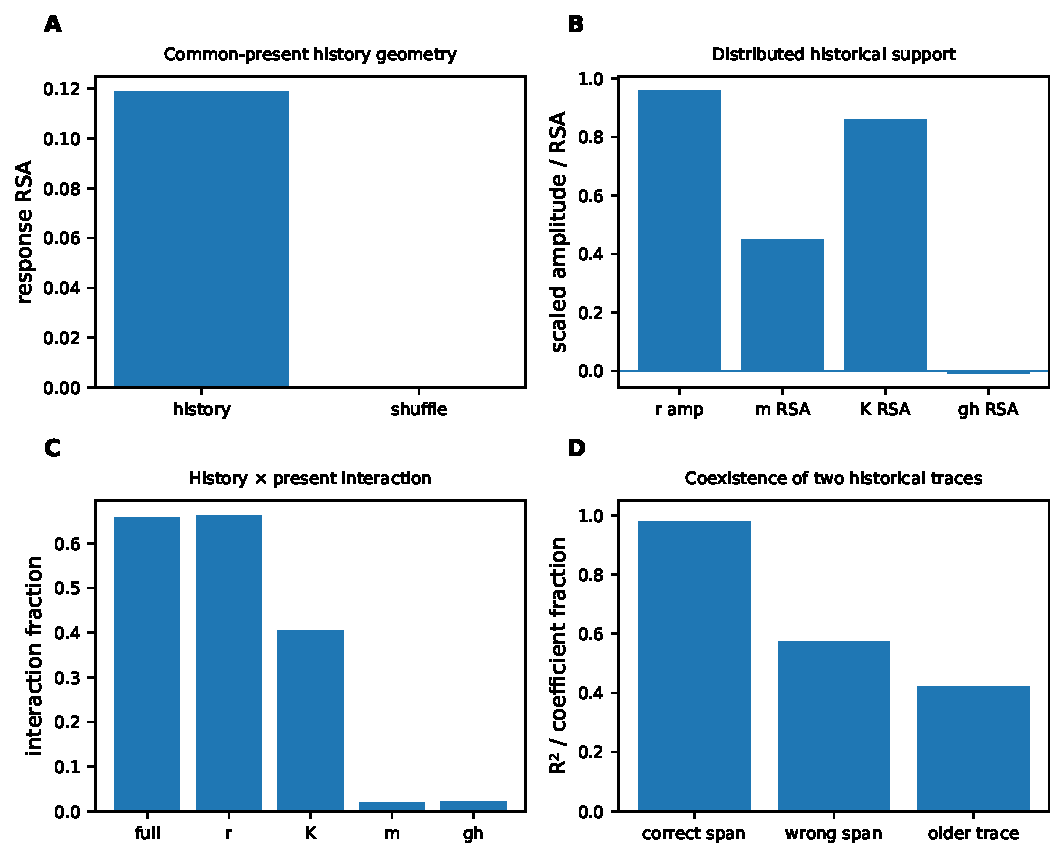
\includegraphics[width=0.96\textwidth]{figures/fig1_history_trace.pdf}
\caption{Historical traces remain causally available at a common present. (A) Historical response geometry exceeds label shuffle. (B) Historical support is distributed: $r$ dominates response amplitude, whereas $K$ and $m$ preserve strong geometry. The $r$ amplitude ratio is shown divided by ten for a common display scale. (C) History-by-present interaction remains large after removing main effects. (D) The correct two-trace span explains later $K$ state substantially better than an unrelated span, while the older trace retains a nontrivial coefficient.}
\label{fig:history}
\end{figure*}

\subsection{Superposed traces are converted into nonlinear operation by collective readout}

A synthetic additive boundary state
\begin{equation}
 K_{\mathrm{synth}}=K_0+(K_A-K_0)+(K_B-K_0)
\end{equation}
closely matched the actual dual-trace state: mean state discrepancy was $0.01514$, and mean response-match error was $0.02034$. Yet synthetic downstream nonadditivity remained large relative to state error: the excess was $0.09776$ (95\% CI $[0.08099,0.11503]$). The actual-versus-synthetic nonadditivity discrepancy was only $0.00401$. Storage was therefore close to additive while downstream operation remained nonlinear.

The principal readout transformation was localized to relative row magnitude and collective centering (Fig.~\ref{fig:readout}). The row-norm residual was $0.06526$; median centering added mean residual $0.03776$, while the sigmoid itself added only approximately $6.7\times10^{-8}$. Replacing endogenous $b$ by the exact additive construction reduced action residual to $3.30\times10^{-7}$, a mean reduction of $0.11629$. A third trace contextually reweighted the previously stored pair, producing mean relative interaction $0.19663$ in $b$ and $0.20488$ in action; the additive-$b$ intervention removed essentially all of both interactions.

We therefore use ``field'' only as a reactor-specific operational shorthand for a distributed historical configuration whose functional meaning is relational. No physical field is implied.

\begin{figure*}[t]
\centering
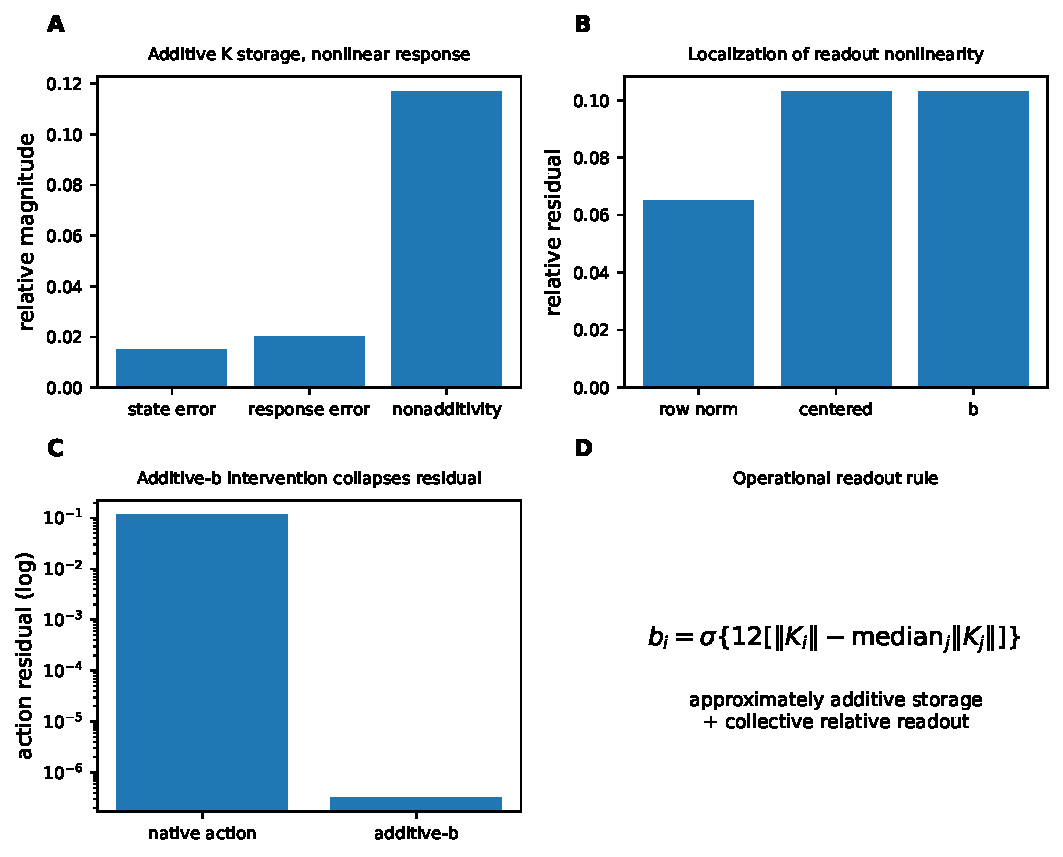
\includegraphics[width=0.96\textwidth]{figures/fig2_storage_readout.pdf}
\caption{Approximately additive storage acquires nonlinear meaning through collective readout. (A) Additive $K$ superposition closely matches the stored state while preserving downstream nonadditivity. (B) Relative row magnitude and median centering localize the principal readout nonlinearity. (C) Replacing endogenous $b$ by an additive construction collapses the action residual on a log scale. (D) Operational boundary readout rule.}
\label{fig:readout}
\end{figure*}

\subsection{Reentry is causal but intrinsically dissipative}

Path dependence survived a closed excursion back to a matched present. The mean excess pairwise response distance of cycle over flat histories was $0.02385$ (95\% CI $[0.02175,0.02591]$), with associated $r$ displacement $0.01565$ and $m$ displacement $0.08395$. The mean non-return mismatch was $0.03446$. Turning-point ablations, reported in the Supplement, showed that both fast and slow state families contributed, with $m$ dominating the slow contribution and $x$ the fast contribution.

Direct perturbation experiments established a bidirectional $x\leftrightarrow m$ relay. The durable $x\rightarrow m$ effect was $0.33948$, an operational fixed-probe relay was $0.31274$, and the $m\rightarrow x$ source-dependence effect was $0.24652$. These results demonstrate causal reentry, but not regenerative recurrence.

An external return-alignment intervention separated geometric fidelity from amplitude loss. At generation 1, aligned return increased target projection by $0.16270$ (95\% CI $[0.14179,0.18557]$); generation-2 rescue was $0.03792$. By generation 3, however, the aligned branch retained only $0.00752$ of the original norm even while directional cosine remained $0.64833$. Geometry could therefore survive after amplitude had almost disappeared.

The isolated full-loop operator made the amplitude limitation explicit. The leading local singular gain was $\sigma_1(T)=0.10188$ at $q_{\mathrm{cal}}$ and $0.10027$ at $q_{\mathrm{test}}$, while finite-amplitude gains along the top mode were $0.09955$ and $0.10025$ (Fig.~\ref{fig:reentry}). No regenerative direction was found in this local carrier regime.

The half-channel factorization showed where the loss arose. Mean write gain was $\sigma_1(A)=0.13158$ at $q_{\mathrm{cal}}$ and $0.13151$ at $q_{\mathrm{test}}$. The return channel was roughly nine times stronger, but the ideal singular-gain products $\sigma_1(A)\sigma_1(B)=0.15782$ and $0.15947$ remained below one. Native interface efficiency was only $0.64764$ and $0.64550$. In this sense, the reactor can return information better than it can preserve it during inscription.

\begin{table}[b]
\caption{Local causal relay geometry and bottleneck. Values are 64-seed means.}
\label{tab:relay}
\begin{ruledtabular}
\begin{tabular}{lcc}
Metric & $q_{\mathrm{cal}}$ & $q_{\mathrm{test}}$\\
\hline
$\sigma_1(T)$ & 0.101877 & 0.100274\\
Finite top-mode gain & 0.099548 & 0.100247\\
$\sigma_1(A)$ & 0.131577 & 0.131510\\
$\sigma_1(B)/\sigma_1(A)$ & 9.25786 & 9.34837\\
$\sigma_1(A)\sigma_1(B)$ & 0.157821 & 0.159474\\
Interface efficiency & 0.647641 & 0.645495\\
\end{tabular}
\end{ruledtabular}
\end{table}

\begin{figure*}[t]
\centering
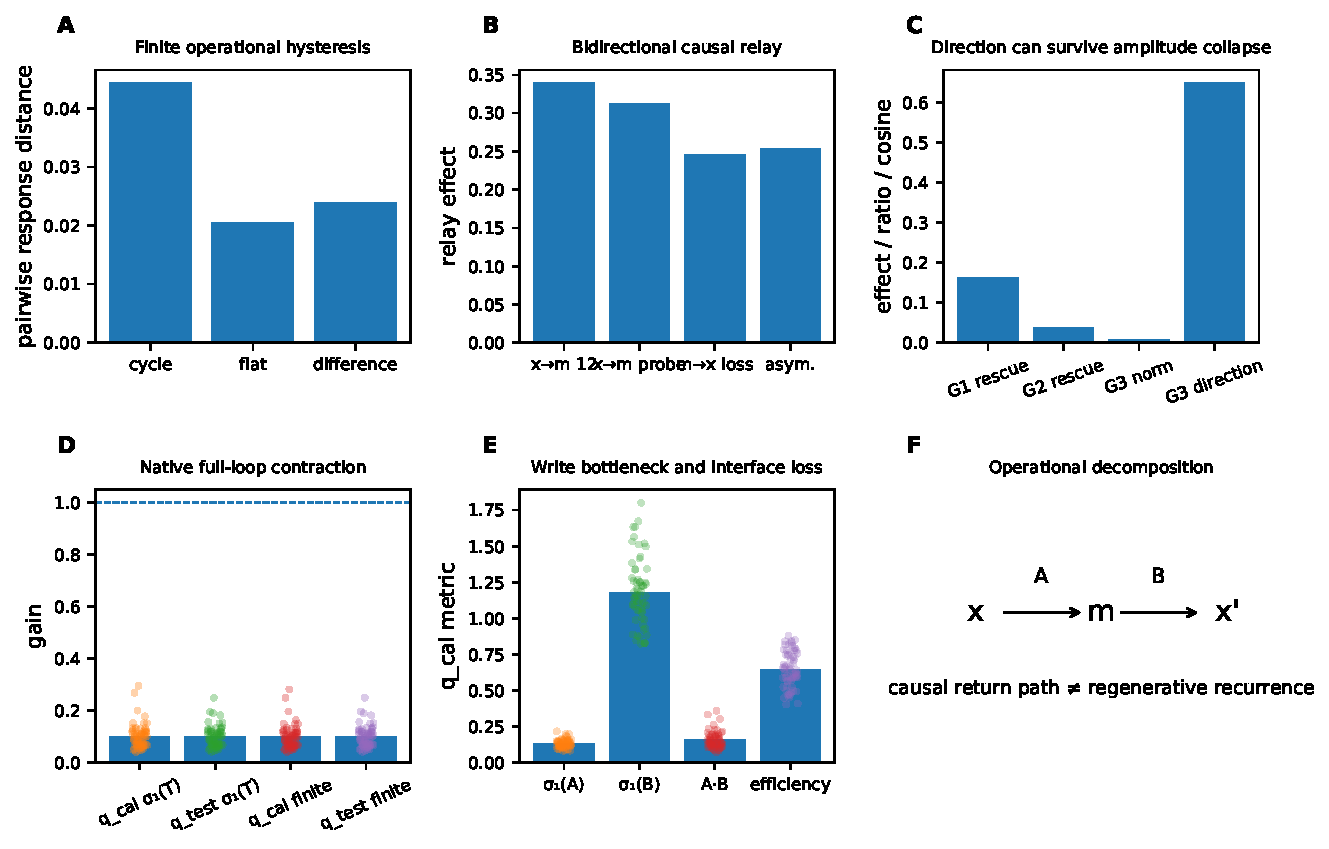
\includegraphics[width=0.98\textwidth]{figures/fig3_reentry.pdf}
\caption{Causal reentry is real but dissipative. (A) Finite operational hysteresis. (B) Bidirectional $x\leftrightarrow m$ relay. (C) External return alignment preserves directional structure while amplitude collapses. (D) The native full loop is locally contractive. (E) Writing is the dominant amplitude bottleneck and native interface geometry adds further loss. (F) Operational half-channel decomposition.}
\label{fig:reentry}
\end{figure*}

\subsection{Selection during transit does not reproduce the selected mode}

Because the native loop was strongly contractive, we first asked whether scalar gain alone would suffice. Setting $\gamma=1/\sigma_1(T_0)$ kept the leading singular value nearly normalized across four generations: mean relative deviation was $0.03339$, with 62 of 64 seeds below $0.20$. Nevertheless, the inherited packet rapidly left the dominant input direction. Mean alignment was $0.99926$ at generation 1 but only $0.29517$ at generation 2, and $84.4\%$ of seeds fell below $0.5$. Reorienting the same-norm packet to the contemporaneous dominant input mode restored mean gain to $0.97972$ over generations 2--4, versus $0.38377$ for the inherited packet. At generation 4 the reoriented norm was $0.95002$, whereas the inherited norm was $0.07998$.

This failure was not caused by a moving target. Consecutive dominant input modes were almost stationary: mean $|\cos(v_g,v_{g+1})|=0.99945$, corresponding to a sign-invariant angle of about $1.34^\circ$, and mean projector distance was $0.03315$. We therefore describe the failure as representational drift of the packet relative to a stable mode, not as modal drift.

The reactor did contain information about modal compatibility. Across equal-norm input perturbations, compatibility with the dominant input mode strongly predicted the magnitude of the resulting $m$ imprint (mean Spearman $\rho=0.92693$), and aligned inputs produced $2.43$ times the memory imprint of orthogonal inputs. A local $x\rightarrow m$ operator predicted this effect almost exactly: mean norm correlation $0.9999972$, mean vector cosine $0.9999976$, and mean relative norm error $0.00104$. Yet an independent 16-seed diagnostic found no reliable evidence that the native system used this signal for modal correction; the tested effects were small and signs were near chance.

One-pass modal competition nevertheless strongly favored the compatible component. Starting from equal compatible and orthogonal energy, compatible share increased from $0.5$ at input to $0.80501$ in memory and $0.86727$ after return. Return therefore added another $0.06226$ of compatible share in 61 of 64 seeds. Selection during the passage was real.

The missing operation was exposed by the input-output singular geometry. Mean $|u_1^Tv_1|=0.315999$ (all seeds $<0.65$), while finite-amplitude output followed $u_1$ with cosine $0.9999985$. The output preference for $u_1$ over $v_1$ was $0.68393$, and $\sigma_1/\rho(T)=2.66303$, with normalized non-normality $0.75534$. Thus the sequence was selection $\rightarrow$ transformation $\rightarrow$ representational drift $\rightarrow$ extinction. Non-normality is part of this mechanism in the tested reactor, but we do not claim that it is the sole universal cause of recurrence failure.

\begin{figure*}[t]
\centering
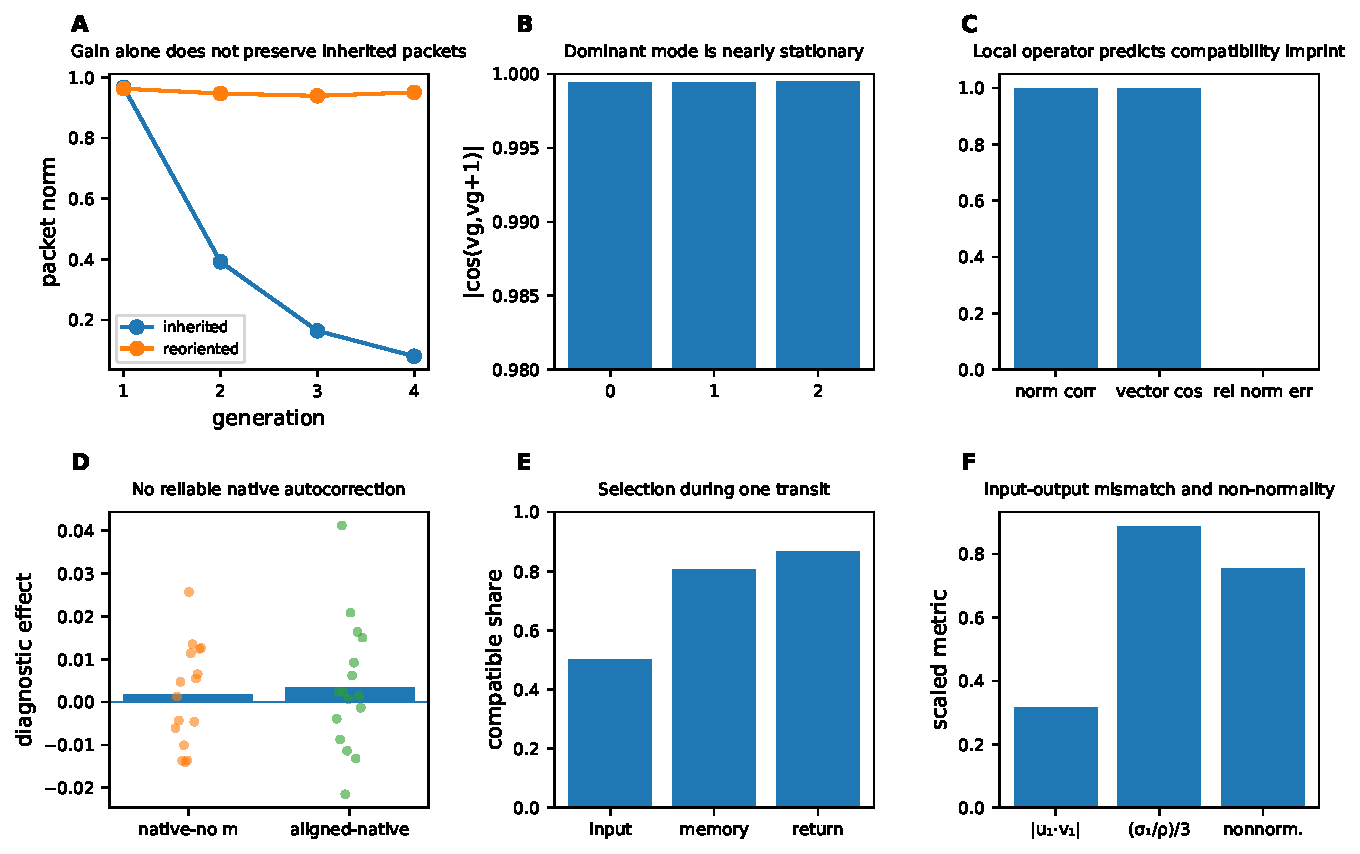
\includegraphics[width=0.98\textwidth]{figures/fig4_selection.pdf}
\caption{Native selection does not reproduce the selected mode. (A) Fixed gain preserves reoriented packets but not inherited output geometry. (B) The dominant input mode is nearly stationary. (C) The local write operator predicts compatibility-dependent memory imprint. (D) No reliable native modal autocorrection was detected in the independent diagnostic. (E) Compatible share is enriched during native write and return. (F) Dominant input and output modes are strongly misaligned and the loop is non-normal; $\sigma_1/\rho$ is divided by three only for the shared display scale.}
\label{fig:selection}
\end{figure*}

\subsection{Closure geometry is captured by instance-specific effective causal dynamics}

We next tested whether closure was already hidden in state variables co-produced with $x$. Restoring all tested non-$x$ co-products changed second-loop gain by only $6.62\times10^{-5}$ in absolute value; mean gain ratio was $0.99993$. Restoring all slow co-products was similarly ineffective. Within the tested variables, carrier, and timescale, no native co-product package supplied the missing output-to-input bridge.

A common closure map across reactor instances also failed in a diagnostic analysis. Mean held-out absolute alignment was $0.23077$ for identity, $0.12746$ for common Procrustes, $0.16025$ for ridge regression, and $0.11840$ for the tested state-conditioned map. In contrast, a simple within-instance orthogonal bridge reconstructed in calibration context transferred to the test context with mean alignment $0.99635$, exceeding identity by $0.69771$ and a wrong-instance map by $0.70759$. Static reciprocity and static subspace/basis hypotheses were then prospectively tested and were insufficient; those negative results are detailed in the Supplement.

The effective causal factorization yielded a much stronger map. The dynamic closure reconstructed once in $c_A$ achieved mean test-context absolute alignment $0.999763$ (all seeds $>0.99$). It exceeded the tested static map by $0.41543$ and a wrong-seed dynamic map by $0.86318$, with all seeds favorable. The mean absolute error in predicting the amount of closure needed in the test context was $0.00276$. The input and output modal frames themselves were highly stable across the context change ($|u_A^Tu_B|\approx0.99895$, $|v_A^Tv_B|\approx0.99900$).

The result supports a narrow statement: closure geometry was accurately captured by the instance-specific effective causal write-return factorization and transferred across the single tested calibration-to-test context change. The map was externally reconstructed and should not be interpreted as an internal computation of the reactor.

As a post-confirmatory robustness audit performed after manuscript review, we repeated the same frozen construction over four symmetry-related calibration-to-test context pairs using the same 64-seed C07 cohort. Across 256 seed--pair cells, mean transferred alignment was $0.999576$; $254/256$ cells exceeded $0.99$. The dynamic map beat the tested static map in every cell by a mean $0.416856$, and closure-need mean absolute error was $0.00461$ ($253/256$ cells below $0.03$). This audit was not prospectively frozen and is not used to redefine the confirmatory C07 outcome; it only tests whether the original transfer was unusually pair-specific.

\begin{figure*}[t]
\centering
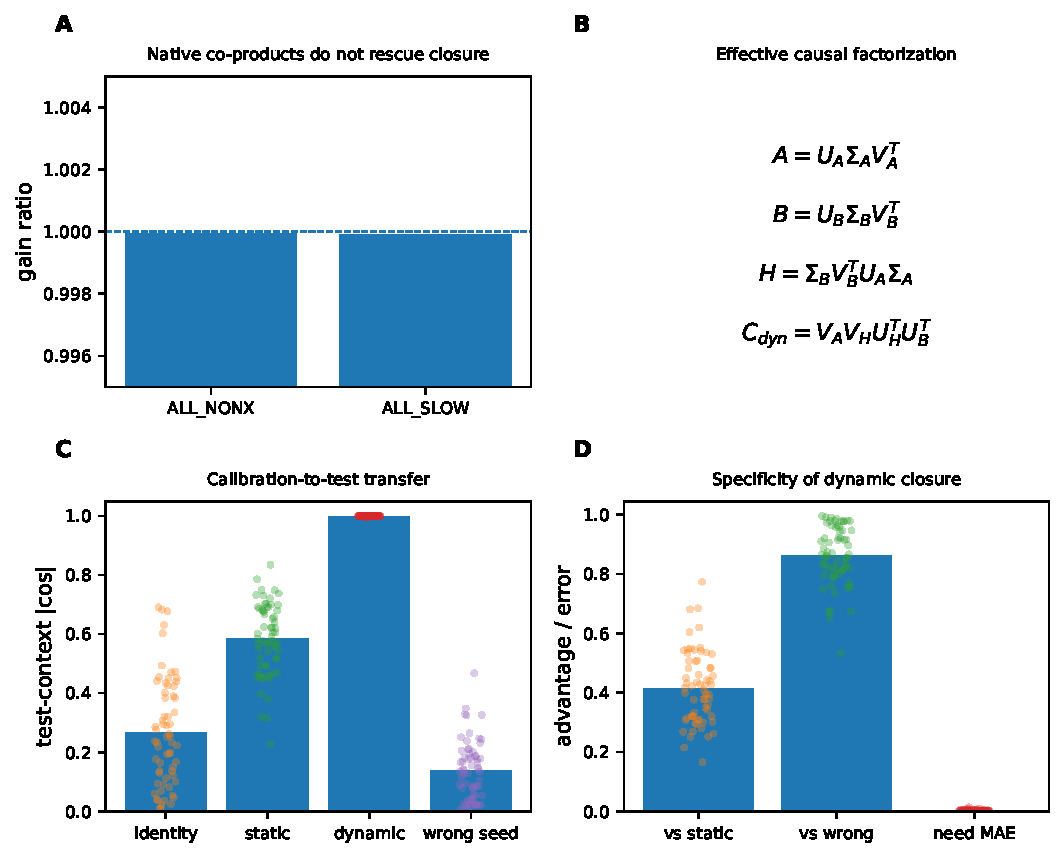
\includegraphics[width=0.96\textwidth]{figures/fig5_closure.pdf}
\caption{Closure is captured by instance-specific effective causal geometry. (A) Native co-produced variables do not rescue second-loop gain. (B) Factorized construction of $\Cdyn$. (C) Calibration-to-test transfer strongly favors the dynamic map. (D) Dynamic closure outperforms the static and wrong-instance controls while predicting test-context closure need with low error.}
\label{fig:closure}
\end{figure*}

\subsection{Fixed closure plus fixed gain is sufficient for finite-horizon regenerative reentry}

The final experiment froze both the instance-specific dynamic closure and the scalar gain in calibration context and evaluated four full nonlinear generations in the distinct test context. The correct fixed intervention preserved mean relative packet norm $0.99440$, $0.99433$, $0.99525$, and $0.99213$ across generations 1--4. The geometrically unclosed control received the same fixed gain but decayed to $0.07959$ by generation 4; the tested static closure reached $0.19929$, and the wrong-instance dynamic closure approximately $0.015$.

The prospectively frozen primary criteria all passed (Table~\ref{tab:confirm}). At generation 4, the correct branch had mean relative norm $0.99213$ with 62 of 64 seeds above $0.70$. Its advantage over the same-gain/no-closure control was $0.91254$ (all seeds favorable), and its advantage over the better of the static and wrong-seed controls was $0.79242$ (all seeds favorable). Mean post-closure alignment over generations 1--4 was $0.999136$, and every seed maintained minimum post-closure alignment above $0.98$. Pre-closure alignment remained near $0.285$, demonstrating that the native return still produced the incompatible geometry that closure was correcting. A post-confirmatory reference-reproduction audit found that the explicit post-closure norm-restoration factor remained within $0.54\%$ of one across all 256 seed--generation packets; disabling that restoration changed reproduced generation-4 mean relative norm by less than $0.001$. Thus the observed persistence is not materially supplied by the norm-restoration step.

A separate projective-basin test used a single frozen kit per seed and mixed packets at four initial angles. Across all nonorthogonal cells, mean generation-4 compatible share was $0.99025$, with $98.96\%$ of cells above $0.90$. For the difficult $67.5^\circ$ condition, compatible share increased by $0.83312$. The fixed-closure advantage over the same-gain geometrically unclosed branch was $0.87315$. At generation 1, the exactly orthogonal $90^\circ$ condition retained only $0.00154$ compatible share, whereas the $67.5^\circ$ condition reached $0.86412$; every seed had greater share in the latter condition. The empirical claim is therefore a finite-horizon projective basin for nonorthogonal packets and absence of immediate attraction from exact orthogonality, not an invariant-subspace theorem or a global nonlinear attractor claim.

\begin{table*}[t]
\caption{Prospectively frozen tests of finite-horizon regenerative reentry. CI denotes bootstrap 95\% interval where applicable.}
\label{tab:confirm}
\centering
\small
\resizebox{\textwidth}{!}{%
\begin{tabular}{llllc}
\toprule
Block & Frozen criterion (abridged) & Observed result & CI & Outcome\\
\midrule
G01 H1 & G4 mean $>0.85$; $>90\%$ seeds $>0.70$ & $0.992131$; fraction $0.96875$ & $[0.960493,1.021435]$ & PASS\\
G01 H2 & correct closure beats same-gain/no-closure by $>0.70$ & $+0.912540$; all seeds positive & $[0.881205,0.941729]$ & PASS\\
G01 H3 & correct geometry beats STATIC/WRONG by $>0.60$ & $+0.792420$; all seeds positive & $[0.756705,0.827210]$ & PASS\\
G01 H4 & mean G1--G4 alignment $>0.99$ & $0.999136$; all seed minima $>0.98$ & -- & PASS\\
G02 H1 & nonorthogonal G4 share $>0.95$ & $0.990252$ & $[0.987357,0.992740]$ & PASS\\
G02 H2 & $67.5^\circ$ enrichment $>0.70$ & $+0.833120$; all positive & $[0.825598,0.839580]$ & PASS\\
G02 H3 & closure advantage $>0.65$ & $+0.873150$; all positive & $[0.860523,0.885624]$ & PASS\\
G02 H4 & $90^\circ$ not immediately attracted & G1: $0.001544$ vs $0.864123$ at $67.5^\circ$ & -- & PASS\\
\bottomrule
\end{tabular}}
\end{table*}

\begin{figure*}[t]
\centering
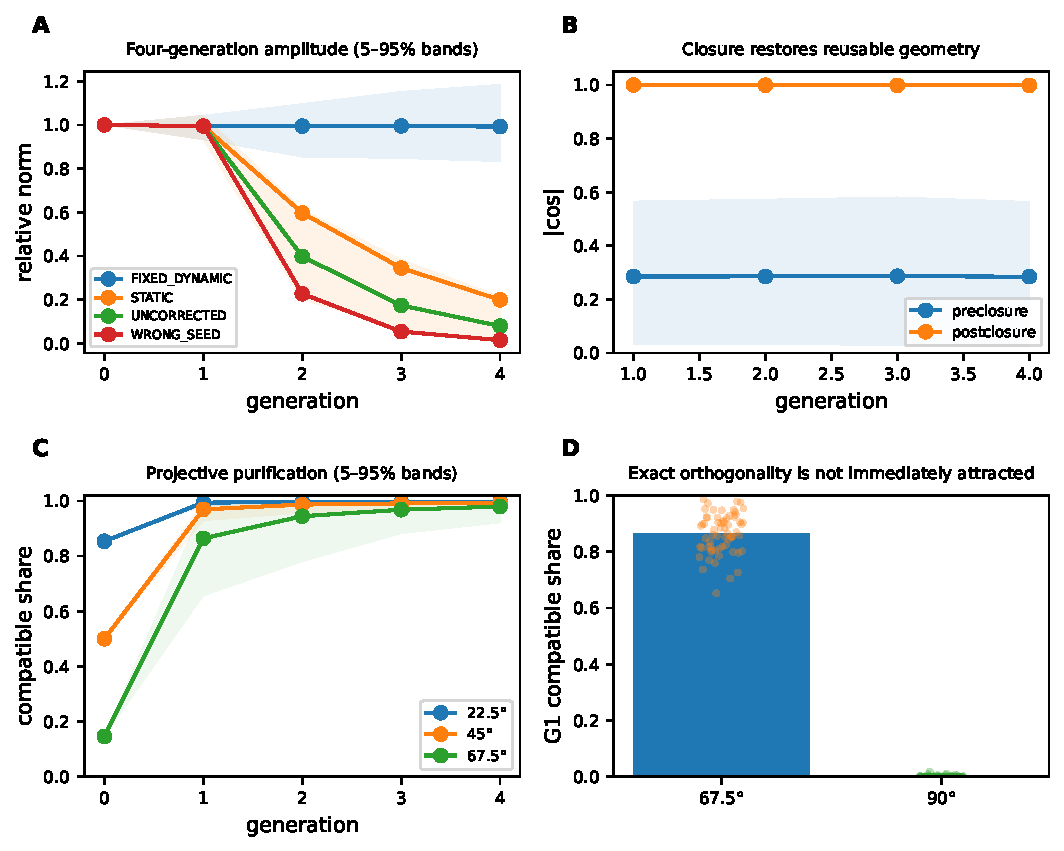
\includegraphics[width=0.96\textwidth]{figures/fig6_regeneration.pdf}
\caption{Fixed modal closure and gain produce finite-horizon regenerative reentry. (A) The frozen dynamic closure preserves near-unit amplitude through four generations, unlike static, wrong-instance, and same-gain/no-closure controls. (B) Returned packets remain weakly aligned before closure and nearly perfectly aligned afterward. (C) Nonorthogonal packets undergo projective purification. (D) Exact orthogonality is not immediately attracted at generation 1.}
\label{fig:regeneration}
\end{figure*}

\section{Discussion}

\subsection{Memory can persist without being reproductively reusable}

The first result is a separation of historical persistence from repeated transmissibility. A past trajectory remains causally active at a matched fast present, and that trace is distributed: different variables carry amplitude, relational geometry, and context sensitivity to different degrees. The boundary matrix $K$, for example, can preserve strong historical geometry while exerting almost no direct response magnitude. The slow memory $m$ and relevance state $r$ contribute differently again. The trace is therefore better described as a distributed historical configuration than as a single storage variable.

This organization becomes operational through collective readout. Approximate local additivity of $K$ does not imply additive behavior because row magnitudes are evaluated relative to their collective median. Historical ``meaning'' in this limited computational sense is therefore relational: the effect of one stored trace depends on the other stored traces and on the present probe.

Causal reentry adds another property but still does not solve recurrence. The $x\rightarrow m\rightarrow x$ path is experimentally real, yet strongly contractive. The existence of a return path is therefore not equivalent to the ability to sustain repeated reuse.

\subsection{Selection during transmission is not reproduction across transmissions}

The native channel preferentially selects compatible components: equal compatible and orthogonal energy becomes strongly enriched toward the compatible component in $m$ and further enriched after return. The system also contains a compatibility-dependent signal in the memory imprint, and a local causal write operator predicts it almost exactly. Nevertheless, we did not detect reliable native use of this signal for modal correction.

The singular geometry clarifies why selection can coexist with extinction. The optimal input direction $v_1$ is transformed into an output direction $u_1$ that is far from $v_1$. Because the dominant input mode itself is nearly stationary, the inherited packet drifts relative to a stable transmission geometry. Scalar gain normalizes magnitude but leaves this directional incompatibility untouched. This is precisely the situation in which one-pass selection is not reproduction across passages.

\subsection{Modal closure is an interface condition}

Modal closure is used here as an operational interface concept: what returns from one passage must be transformed into geometry compatible with the next input. The algebraic ingredient is deliberately classical: $VU^T$ is closely related to orthogonal Procrustes and polar-factor constructions \cite{Schonemann1966,Higham1986}. The empirical contribution is therefore not the existence of a rotation between two orthonormal frames. It is the causal identification of the relevant write--return frames in a nonlinear adaptive simulator, the freezing of the resulting instance-specific map, and its intervention-level transfer to a distinct context. Similarly, loop-gain language provides useful intuition for amplitude sufficiency \cite{Zames1966}, but the finite-horizon nonlinear result is established by direct intervention rather than by applying a general feedback-stability theorem. The tested native co-product packages did not supply such a bridge. A common map across random reactor instances also failed, and simple reciprocity or static subspace/basis hypotheses were insufficient. These negatives narrow the mechanism rather than serving as discarded analyses.

The successful map instead came from the effective causal dynamics of the two half-channels. Its calibration-to-test transfer is important because same-carrier alignment is partly built into the singular-vector construction. In the distinct test context, the frozen dynamic map reached $0.999763$ mean alignment and strongly outperformed static and wrong-instance controls. Still, only one calibration-to-test pair was tested; broader context generalization remains open.

\subsection{Gain and closure jointly support finite-horizon regenerative reentry}

The final experiment isolates the role of geometry as cleanly as the current design permits because every final branch receives the same fixed scalar gain. The strongest contrast is therefore not ``corrected versus native,'' but correct fixed closure versus the same fixed gain with no geometric closure. Within this repaired protocol, finite-horizon recurrence depended strongly on geometric compatibility: correct closure maintained near-unit amplitude and reusable direction, while the gain-compensated but geometrically unclosed branch decayed by more than an order of magnitude.

The projective-basin experiment provides an additional mechanistic check. Nonorthogonal mixtures are progressively purified toward the compatible mode under the frozen repair. An exactly orthogonal packet is not immediately attracted, matching the ideal fixed-linear prediction at the first generation. Because later nonlinear generations can create compatible components, no stronger invariant-subspace claim is made.

``Regenerative'' therefore has a strictly operational meaning here: persistence of transmissible organization over four externally corrected generations. The system neither learns nor energetically maintains the correction.

\subsection{Limitations and next question}

The main limitations are explicit. First, $A$, $B$, and $T$ are local causal operators tied to defined carriers, interventions, and finite windows. Second, the nonlinear endpoint is four generations, not an asymptotic stability proof. Third, the prospectively frozen closure-transfer test used one calibration-to-test context pair. A post-confirmatory same-cohort audit over four symmetry-related pairs was strongly consistent with broader transfer, but it is not an independent confirmatory multi-context replication. Fourth, exact orthogonality was only tested for immediate attraction and later nonlinear dynamics are not constrained by the ideal linear argument. Fifth, gain and closure were externally reconstructed and frozen; the reactor does not infer them from its own consequences.

The public reproduction release also distinguishes scientific reproducibility from forensic source recovery. The base reactor, frozen designs, result tables, and six late-stage scripts are preserved as original artifacts or verbatim transcript recovery. Three transient dependencies were not recovered byte-identically; validated reference reconstructions are released separately. Their operator outputs preserve the frozen confirmatory conclusions, but the original transient noise-seed mixer was not independently archived, so exact seedwise equality of every auxiliary column is not claimed.

The natural next question is therefore not whether an external closure can work, but whether a system can acquire the geometry of return from causal consequences without an external singular-value oracle. That question lies outside the present paper.

\section{Conclusion}

Historical persistence, causal return, and one-pass selection are each insufficient for repeated reuse in the tested adaptive reactor. The decisive obstruction is an interface mismatch: the geometry emitted by one passage is not the geometry best transmitted by the next. A closure map constructed from effective causal write and return dynamics, when frozen and combined with fixed gain normalization, is sufficient to produce four generations of nonlinear regenerative reentry and projective purification of nonorthogonal packets. The result is finite-horizon, externally repaired, instance specific, and computational. It does not establish autonomous learning or asymptotic self-maintenance.

\section*{Data and code availability}

The public repository associated with this preprint contains the manuscript source, figures and figure-generation script, archived result tables, recovered frozen designs, original base-reactor code, transcript-recovered late-stage runners, validated reference reconstructions of three transient dependencies, an experiment-by-experiment execution-coverage table, reconstruction-validation documentation, and SHA-256 manifests. Raw conversation-export files used during source recovery are not distributed publicly because they contain material unrelated to the scientific release; provenance hashes and recovery reports are retained instead. A Zenodo DOI will be attached to the tagged public release.

\section*{Author contributions}

G.R.F.: conceptualization, methodology, software, formal analysis, investigation, visualization, data curation, writing, and project administration.

\section*{AI-assisted workflow disclosure}

OpenAI ChatGPT was used during parts of the longitudinal research organization, manuscript preparation, code recovery from frozen research transcripts, and construction of the reproducibility package. Model versions were not consistently recorded throughout the full research history; the final release audit and manuscript assembly used GPT-5.6 Sol. The author directed the system by supplying frozen design records, source code, result tables, explicit falsification constraints, and requests for adversarial consistency checks. AI-assisted outputs were verified against recovered source files, primary result tables, executable reruns, and archived numerical outputs; reconstructed code is explicitly labeled by provenance. Scientific decisions, interpretation, authorship, and responsibility for the work remain with the author.

\begin{thebibliography}{99}
\bibitem{Ganguli2008} S. Ganguli, D. Huh, and H. Sompolinsky, Memory traces in dynamical systems, Proc. Natl. Acad. Sci. USA \textbf{105}, 18970 (2008), doi:10.1073/pnas.0804451105.
\bibitem{Goldman2009} M. S. Goldman, Memory without feedback in a neural network, Neuron \textbf{61}, 621 (2009), doi:10.1016/j.neuron.2008.12.012.
\bibitem{Maass2002} W. Maass, T. Natschl\"ager, and H. Markram, Real-time computing without stable states: A new framework for neural computation based on perturbations, Neural Comput. \textbf{14}, 2531 (2002), doi:10.1162/089976602760407955.
\bibitem{JaegerHaas2004} H. Jaeger and H. Haas, Harnessing nonlinearity: Predicting chaotic systems and saving energy in wireless communication, Science \textbf{304}, 78 (2004), doi:10.1126/science.1091277.
\bibitem{Lukosevicius2009} M. Luko\v{s}evi\v{c}ius and H. Jaeger, Reservoir computing approaches to recurrent neural network training, Comput. Sci. Rev. \textbf{3}, 127 (2009), doi:10.1016/j.cosrev.2009.03.005.
\bibitem{Mante2013} V. Mante, D. Sussillo, K. V. Shenoy, and W. T. Newsome, Context-dependent computation by recurrent dynamics in prefrontal cortex, Nature \textbf{503}, 78 (2013), doi:10.1038/nature12742.
\bibitem{Rigotti2013} M. Rigotti, O. Barak, M. R. Warden, X.-J. Wang, N. D. Daw, E. K. Miller, and S. Fusi, The importance of mixed selectivity in complex cognitive tasks, Nature \textbf{497}, 585 (2013), doi:10.1038/nature12160.
\bibitem{Sussillo2009} D. Sussillo and L. F. Abbott, Generating coherent patterns of activity from chaotic neural networks, Neuron \textbf{63}, 544 (2009), doi:10.1016/j.neuron.2009.07.018.
\bibitem{Laje2013} R. Laje and D. V. Buonomano, Robust timing and motor patterns by taming chaos in recurrent neural networks, Nat. Neurosci. \textbf{16}, 925 (2013), doi:10.1038/nn.3405.
\bibitem{Trefethen2005} L. N. Trefethen and M. Embree, \textit{Spectra and Pseudospectra: The Behavior of Nonnormal Matrices and Operators} (Princeton University Press, Princeton, 2005).
\bibitem{Hennequin2014} G. Hennequin, T. P. Vogels, and W. Gerstner, Optimal control of transient dynamics in balanced networks supports generation of complex movements, Neuron \textbf{82}, 1394 (2014), doi:10.1016/j.neuron.2014.04.045.
\bibitem{Schonemann1966} P. H. Sch\"onemann, A generalized solution of the orthogonal Procrustes problem, Psychometrika \textbf{31}, 1 (1966), doi:10.1007/BF02289451.
\bibitem{Higham1986} N. J. Higham, Computing the polar decomposition---with applications, SIAM J. Sci. Stat. Comput. \textbf{7}, 1160 (1986), doi:10.1137/0907079.
\bibitem{Zames1966} G. Zames, On the input-output stability of time-varying nonlinear feedback systems Part one: Conditions derived using concepts of loop gain, conicity, and positivity, IEEE Trans. Autom. Control \textbf{11}, 228 (1966), doi:10.1109/TAC.1966.1098316.
\bibitem{Ljung1999} L. Ljung, \textit{System Identification: Theory for the User}, 2nd ed. (Prentice Hall PTR, 1999).
\bibitem{Schmid2010} P. J. Schmid, Dynamic mode decomposition of numerical and experimental data, J. Fluid Mech. \textbf{656}, 5 (2010), doi:10.1017/S0022112010001217.
\end{thebibliography}

\end{document}
